\documentclass[a4paper,12pt]{scrartcl}
\usepackage[utf8x]{inputenc}
\usepackage[T1]{fontenc} % avec T1 comme option  d'encodage c'est ben mieux, surtout pour taper du français.
%\usepackage{lmodern,textcomp} % fortement conseillé pour les pdf. On peut mettre autre chose : kpfonts, fourier,...
\usepackage[french]{babel} %Sans ça les guillemets, amarchpo
\usepackage{amsmath}
\usepackage{multicol}
\usepackage{amssymb}
\usepackage{tkz-tab}
\usepackage{exercice_sheet}
\usepackage{pgf,tikz}
\usepackage{mathrsfs}
\usetikzlibrary{arrows}

%\trait
%\section*{}
%\exo{}
%\question{}
%\subquestion{}


% Title Page
\title{Exercices, exponentielle et logarithme}
%\subtitle{Factorisation, développement, racines carrées et bien d'autres...}
\author{Patrick \textsc{Augeau}}

\begin{document}

\maketitle

%\begin{multicols}{2}

\exo{}

\question{OL uniquement}

\littlestar{En $+\infty$}

$$\lim_{t\to+\infty} e^t = +\infty$$
Or, $e^t + 1 > e^t$ d'où:$\lim\limits_{t\to+\infty} e^t+1 = +\infty$
donc
$$\lim_{t\to+\infty} 2(e^t+1) = +\infty$$
Il s'agit de la forme $\frac{1}{+\infty}$. 
On en déduit donc: 
$$\lim_{t\to+\infty} \dfrac{1}{2(e^t+1)} = 0$$
De façon évidente:
$$\lim_{t\to+\infty} t = +\infty$$
Cette limite est de la forme $0+\infty$, d'où:
$$\lim_{t\to+\infty} g(t) = +\infty$$

\littlestar{En $-\infty$}

$\lim\limits_{t\to-\infty} e^t = 0$ d'où $\lim\limits_{t\to-\infty} e^t + 1 = 1$ et $\lim\limits_{t\to-\infty} 2(e^t + 1) = 2$.

Par passage à l'inverse, $\lim\limits_{t\to-\infty} \dfrac{1}{2(e^t + 1)} = \dfrac{1}{2}$.

De plus, $\lim\limits_{t\to-\infty} t = -\infty$. On est donc dans le cas $-\infty + k$. 

D'où $\lim\limits_{t\to-\infty} g(t) = -\infty$.

\question{}

$g(t) = t + \dfrac{1}{2(e^t+1)}$. La partie fractionnaire est de la forme $\left( \dfrac{1}{u} \right)' = -\dfrac{u'}{u^2}$ avec $u(t) = 2(e^t + 1)$ et $u'(t) = 2e^t$. 

La dérivée de $t$ est 1.

D'où $g'(t) = 1 - \dfrac{2e^t}{4(e^t+1)^2} = 1 - \dfrac{e^t}{2(e^t+1)^2}$.

Par mise au même dénominateur, on obtient $g'(t) = \dfrac{2(e^t+1)^2 - e^t}{2(e^t+1)^2} = \dfrac{2(e^{2t} + 2e^t + 1) - e^t}{2(e^t+1)^2}$.

On obtient finalement, par simplification: $\dfrac{2e^{2t} + 3e^t + 2}{2(e^t+1)^2}$.

\question{}

Afin de dresser le tableau de variation de g, il  faut nous intéresser au signe de $g'$ car c'est lui qui va nous indiquer les variations de $g$.

\littlestar{Signe du numérateur}

Quel que soit $t \in \mathbb{R}$, 
$e^t > 0$. Il s'agit d'une somme de nombres strictement positifs. Le numérateur de $g(t)$ est donc strictement positif sur $\mathbb{R}$.

\littlestar{Signe du dénominateur}

$$e^t > 0$$
$$\Leftrightarrow e^t+1 > 1$$
$$\Leftrightarrow (e^t + 1)^2 > 1^2$$
$$\Leftrightarrow 2(e^t + 1)^2 > 2$$

$g'(t)$ est donc le quotient de deux nombres strictement positifs et est donc strictement positive pour $t \in \mathbb{R}$. $g$ est donc strictement croissante sur $\mathbb{R}$.

\begin{center}
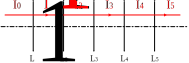
\includegraphics[width=0.5\textwidth]{pics/1.png}
\end{center}

\exo{$h(t) = e^{2t} - 7e^t + 5t + 1$}

\question{}

$h'(t) = 2e^{2t} - 7e^t + 5$. Le plus simple est de développer l'expression donnée dans l'énoncé. 

$$(e^t - 1)(2e^t-5) = 2e^{2t} - 5e^t - 2e^t + 5 = 2e^{2t} - 7e^t + 5$$.

\question{}

\subquestion{}

Afin d'étudier le signe, nous allons utiliser la forme factorisée de: $$h'(t) = (e^t-1)(2e^t-5)$$.

\littlestar{d'une part}

$$e^t-1 \geq 0$$ %***
$$\Leftrightarrow e^t \geq 1$$
$$\Leftrightarrow \ln(e^t) \geq \ln(1)$$
$$\Leftrightarrow t \geq 0$$.

Précision: le raisonnement est ici fait par équivalences. Il peut se résumer en une seule étape: $e^t-1 \geq 0 \Leftrightarrow t \geq 0$. Cela signifie que lorsque $t$ est positif, $e^t - 1$ est positif, mais aussi que lorsque $t$ n'est pas positif (donc négatif), $e^t - 1$ est négatif. Cela va nous permettre de remplir la ligne du tableau de signe correspondant à $e^t - 1$. 

\littlestar{D'autre part}

$$2e^t - 5 \geq 0$$
$$\Leftrightarrow 2e^t \geq 5$$
$$\Leftrightarrow e^t \geq \dfrac{5}{2}$$
$$\Leftrightarrow t \geq \ln \left( \dfrac{5}{2} \right)$$

On peut donc dresser le tableau de signe suivant:

\begin{center}
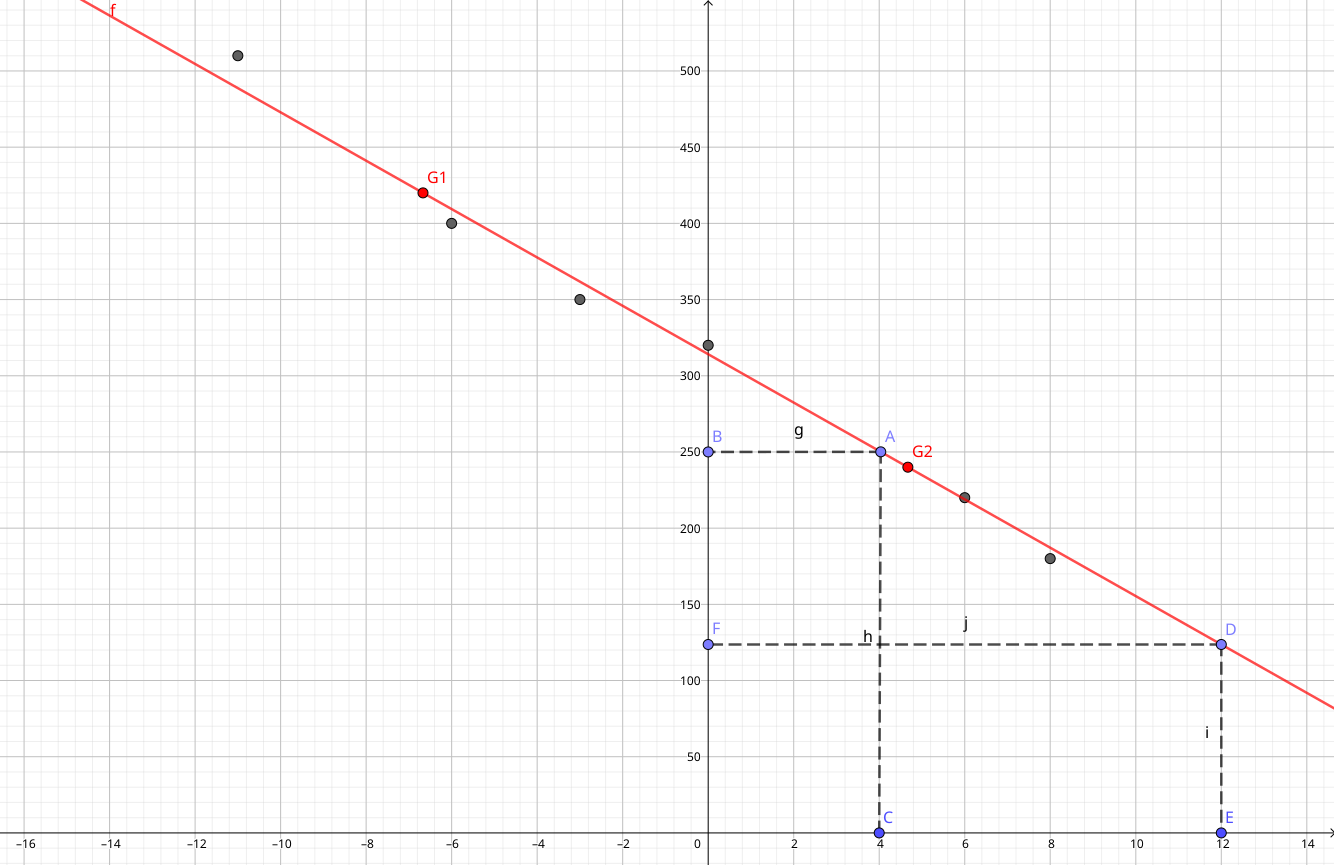
\includegraphics[width=0.5\textwidth]{pics/2.png}
\end{center}

\subquestion{}

$$h(0) = 1^2 - 7 + 1 = -5$$

$$h\left(\ln\left(\dfrac{5}{2}\right)\right) = \left( \dfrac{5}{2} \right)^2 - 7 \times \dfrac{5}{2} + 5 \ln\left( \ln \dfrac{5}{2} \right)$$.

Donc $h\left(\ln\left(\dfrac{5}{2}\right)\right) = -\dfrac{41}{4} + 5 \ln \dfrac{5}{2} \approx -5.67$.

On en déduit le tableau de variation suivant:

%[Tableau de variations]
\begin{center}
\includegraphics[width=0.5\textwidth]{pics/3.png}
\end{center}

\exo{}

\question{OL uniquement}

\littlestar{En $+ \infty$}

$\lim\limits_{t\to+\infty} \ln t = +\infty$ et $\lim\limits_{t\to+\infty} -t = -\infty$.

On a donc une forme indéterminée. Afin de la lever, on factorise $f(t)$ par $t$:

$$f(t) = t \left( \dfrac{\ln(t)}{t} - \dfrac{t}{t} - \dfrac{1}{t} \right) = t \left( \dfrac{\ln(t)}{t} - 1 - \dfrac{1}{t} \right)$$. 

De par le théorème des croissances comparées, on sait que $\lim\limits_{t\to+\infty} \dfrac{\ln(t)}{t} = 0$.

De plus, $\lim\limits_{t\to+\infty} \dfrac{1}{t} = 0$,

et $\lim\limits_{t\to+\infty} -1 = -1$.

Donc $\lim\limits_{t\to+\infty} \left( \dfrac{\ln(t)}{t} - 1 - \dfrac{1}{t} \right) = -1$

\littlestar{En $0^+$}

$\lim\limits_{t\to 0^+} \ln t = -\infty$. Ceci est une propriété de la fonction $\ln $, logarithme népérien.

$\lim\limits_{t\to 0^+} -t-1 = -1$. 

Il n'y a pas de forme indéterminée: $\lim\limits_{t\to 0^+} f(t) = -\infty$.

\question{Dérivée}

$f'(t) = \dfrac{1}{t} - 1 = \dfrac{1-t}{t}$.

\question{Tableau de variation}

$$1-t \geqslant 0$$

$$\Leftrightarrow t \leqslant 1$$

En découle le tableau de variation suivant:

\begin{center}
\includegraphics[width=0.5\textwidth]{pics/4.png}
\end{center}

\probleme{}

\partie{}

\question{En $x = 1$}

$g(1) = 1^2 - 1 + \ln(1) = 0$ (note: $\ln(1) = 0$).

\question{Sens de variation de $g$}

$x \longmapsto x^2$ est strictement croissante sur $]0 ; +\infty[$ (rappel, cet ensemble peut aussi s'écrire $\mathbb{R}^{+*}$ où le $+$ signifie positifs et $*$ signifie qu'on retire 0 de l'ensemble).

$x \longmapsto \ln(x)$ est également strictement croissante sur $]0 ; +\infty[$ (propriété de la fonction $\ln$).

$x \longmapsto -1$ est constante sur $\mathbb{R}$, donc sur $]0 ; +\infty[$.

$g$ est donc la somme d'une fonction constante et de 2 fonctions strictement croissantes et est donc strictement croissante sur $]0 ; +\infty[$. 

\question{Signe de $g$}

Comme montré précédemment, $g$ est strictement croissante sur $]0 ; +\infty[$ et $g(1) = 0$.

Ainsi: 

\littlestar{Pour $x < 1$}

$g(x) < g(1)$ (définition d'une fonction croissante).

D'où $g(x) < 0$, donc strictement négatif.

\littlestar{Pour $x > 1$}

$g(x) > g(1)$.

D'où $g(x) > 0$, donc strictement positif.

\partie{}

\question{OL uniquement}

$\lim\limits_{x\to+\infty} \dfrac{\ln(x)}{x} = 0$ (croissances comparées).

$\lim\limits_{x\to+\infty} x-1 = +\infty$.

Il n'y a pas de forme indéterminée: $\lim\limits_{x\to+\infty} f(x) = +\infty$.

\question{Dérivée de $f$}

On reconnaît ici la forme $\left( \dfrac{u}{v} \right)' = \left( \dfrac{u'v - uv'}{v^2} \right)$.

$f'(x) = 1- \dfrac{\frac{1}{x} \times x - \ln x \times 1}{x^2}$.

Par mise au même dénominateur et réduction, on obtient $f'(x) = \dfrac{x^2 - 1 + \ln x}{x^2} = \dfrac{g(x)}{x^2}$.

\question{}

Pour $x > 0$, $x^2 > 0$. $f'(x)$ est donc du signe de $g(x)$ trouvé précédemment. 

On en déduit le tableau de variation de $f$ :

\begin{center}
\includegraphics[width=0.5\textwidth]{pics/5.png}
\end{center}

\question{}

\subquestion{OL uniquement}

Afin d'étudier l'écart entre la courbe et la droite $(D)$, on étudie en $+\infty$ la limite de $f(x) - (x-1)$. 

$f(x) - (x-1) = -\dfrac{\ln x}{x}$ or $\lim\limits_{x\to+\infty} \dfrac{\ln(x)}{x} = 0$ (croissances comparées).

Donc $\lim\limits_{x\to+\infty} f(x) - (x-1) = 0$. 

$(D)$ est donc bien asymptote à $C$ en $+\infty$.

\subquestion{Position relative de la courbe par rapport à la droite, OL uniquement}

On remarque qu'en $+\infty$:

$-\dfrac{\ln x}{x} < 0$

$\Leftrightarrow f(x) - (x-1) < 0$

$\Leftrightarrow f(x) < x-1$

La droite $(D)$ est donc \emph{au dessus} de $C$.

\question{Tableau de valeurs et courbe}

\subquestion{}

$$
\begin{array}{r|c|c|c|c|c|c|c|c}
x & 0,25 & 0,5 & 1 & 2 & e & 4 & 6 & 8\\
\hline
f(x) & 4,8 & 0,9 & 0 & 0,7 & 1,4 & 2,7 & 4,7 & 6,7
\end{array}
$$

\subquestion{}

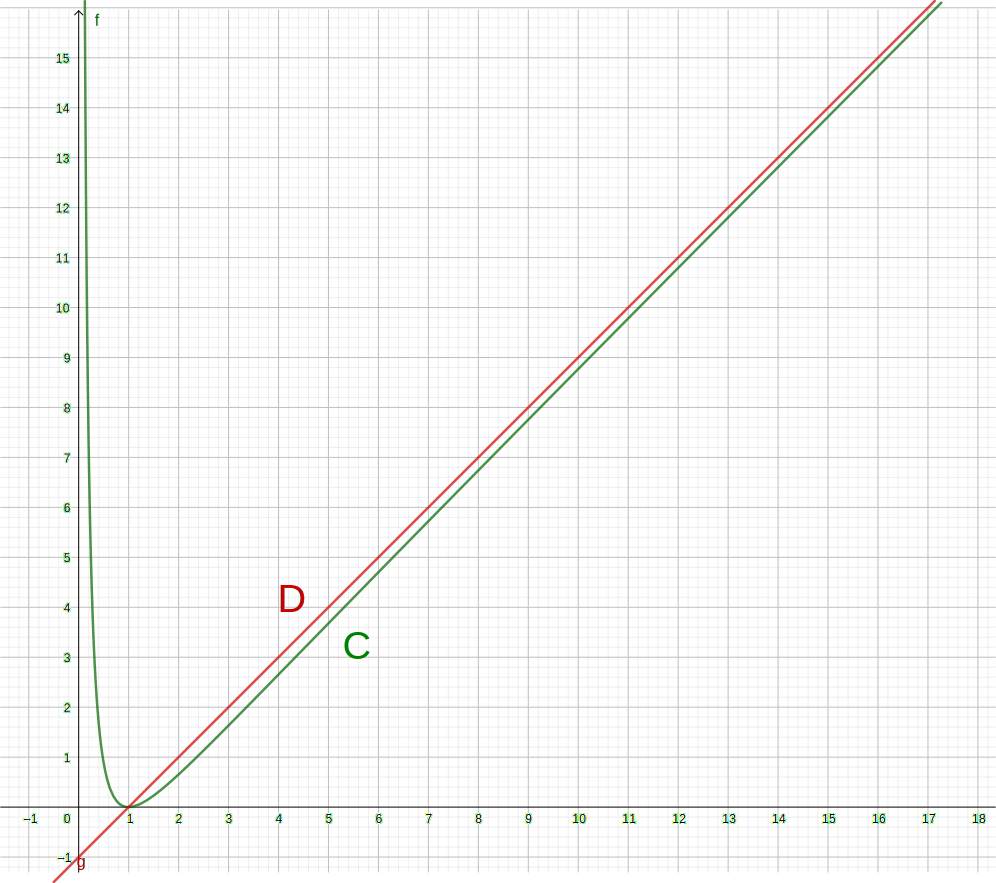
\includegraphics[width=\textwidth]{pics/probleme_last.pdf}

\end{document}